\section{Differentialrechnung}
Sei \(f(x) : D \to \mathbb{R}\) eine Funktion. Die Ableitung \(f'(x_0)\) beschreibt die Änderungsrate der Funktion an der Stelle \(x_0\). Sie wird definiert als der Grenzwert des Differenzenquotienten:
\[
    f'(x_0) = \lim_{\Delta x \to 0} \frac{f(x_0 + \Delta x) - f(x_0)}{\Delta x} = \lim_{x \to 0} \frac{\Delta f}{\Delta x}(x_0) 
\]
\begin{center}
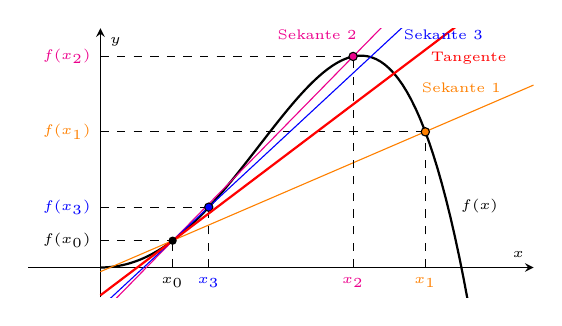
\begin{tikzpicture}[font=\tiny]
    \pgfplotsset{ticks=none}
    \begin{axis}
        [axis lines = middle,
        xlabel = \(x\),
        ylabel = \(y\),
        samples=100,
        ymin=-0.1, ymax=0.8,
        xmin=-0.2, xmax=1.2,
        width=8cm,
        height=5cm
        ]
        \node[above] at (axis cs:1.05,0.15) {\(f(x)\)};
        \addplot[domain=0:1.2, thick] { -4*x^4+2*x^3+2*x^2 };

        \draw[dashed, thin] (axis cs:0.9,0) node[below, orange] {$x_1$} -- (axis cs:0.9, { -4*0.9^4+2*0.9^3+2*0.9^2 });
        \draw[dashed, thin] (axis cs:0,{ -4*0.9^4+2*0.9^3+2*0.9^2 }) node[left, orange] {$f(x_1)$} -- (axis cs:0.9, { -4*0.9^4+2*0.9^3+2*0.9^2 });
        \addplot[domain=0:1.2, thin, orange] {0.520*x -0.014};
        \fill[draw=black, fill=orange] (axis cs:0.9, { -4*0.9^4+2*0.9^3+2*0.9^2 }) circle(1.5pt);
        
        \draw[dashed, thin] (axis cs:0.70,0) node[below, magenta] {$x_2$} -- (axis cs:0.70, { -4*0.70^4+2*0.70^3+2*0.70^2 });
        \draw[dashed] (axis cs:0,{ -4*0.70^4+2*0.70^3+2*0.70^2 }) node[left, magenta] {$f(x_2)$} -- (axis cs:0.70, { -4*0.70^4+2*0.70^3+2*0.70^2 });
        \addplot[domain=0:1.2, thin, magenta] {1.232*x -0.157};
        \fill[draw=black, fill=magenta] (axis cs:0.70, { -4*0.70^4+2*0.70^3+2*0.70^2 }) circle(1.5pt);
        
        \draw[dashed, thin] (axis cs:0.3,0) node[below, blue] {$x_3$} -- (axis cs:0.3, { -4*0.3^4+2*0.3^3+2*0.3^2 });
        \draw[dashed] (axis cs:0,{ -4*0.3^4+2*0.3^3+2*0.3^2 }) node[left, blue] {$f(x_3)$} -- (axis cs:0.3, { -4*0.3^4+2*0.3^3+2*0.3^2 });
        \addplot[domain=0:1.2, thin, blue] {1.120*x -0.134};
        \fill[draw=black, fill=blue] (axis cs:0.3, { -4*0.3^4+2*0.3^3+2*0.3^2 }) circle(1.5pt);
        
        \draw[dashed, thin] (axis cs:0.2,0) node[below] {$x_0$} -- (axis cs:0.2, { -4*0.2^4+2*0.2^3+2*0.2^2 });
        \draw[dashed, thin] (axis cs:0,{ -4*0.2^4+2*0.2^3+2*0.2^2 }) node[left] {$f(x_0)$} -- (axis cs:0.2, { -4*0.2^4+2*0.2^3+2*0.2^2 });
        \addplot[domain=0:1.2, thick, red] {0.912*x -0.093};
        \fill[black] (axis cs:0.2,{ -4*0.2^4+2*0.2^3+2*0.2^2 }) circle(1.5pt);
        
        \node[red] at (axis cs:1.02,0.7) {Tangente};
        \node[orange] at (axis cs:1,0.6) {Sekante 1};
        \node[magenta] at (axis cs:0.6,0.78) {Sekante 2};
        \node[blue] at (axis cs:0.95,0.78) {Sekante 3};
    \end{axis}
\end{tikzpicture}
\end{center}
    
\subsection{Ableitungsregeln}
\begin{itemize}
    \item \textbf{Faktorregel:} \((c \cdot f)'(x) = c \cdot f'(x)\)
    \item \textbf{Summenregel:} \((f + g)'(x) = f'(x) + g'(x)\)
    \item \textbf{Produktregel:} \((f \cdot g)'(x) = f'(x) \cdot g(x) + f(x) \cdot g'(x)\)
    \item \textbf{Quotientenregel:} \(\left(\frac{f}{g}\right)'(x) = \frac{f'(x) \cdot g(x) - f(x) \cdot g'(x)}{(g(x))^2}\)
    \item \textbf{Kettenregel:} \((f \circ g)'(x) = f'(g(x)) \cdot g'(x)\)
\end{itemize}

\subsection{Wichtige Ableitungen}
\begin{align*}
    (x^n)' &= n \cdot x^{n-1} \quad\text{ für } n \in \mathbb{R} \\
    (e^x)' &= e^x \\
    (\ln x)' &= \frac{1}{x} \quad \text{ für } x > 0 \\
    (\log_a x)' &= \frac{1}{x \ln a} \quad \text{ für } x > 0, a > 0, a \neq 1 \\
    (\sin x)' &= \cos x \\
    (\cos x)' &= -\sin x \\
\end{align*}

\subsection{Differenzierbarkeit}
Eine Funktion \(f(x)\) ist an der Stelle \(x_0\) differenzierbar, wenn die links- und rechtsseitigen Ableitungen übereinstimmen. Differenzierbarkeit impliziert Stetigkeit, aber nicht umgekehrt.\\
\emph{Definition:} Eine Funktion heisst differenzierbar, wenn die Ableitung an jeder Stelle ihres Definitionsbereichs existiert.

\subsection{Tangenten- und Normalengleichung}
Die Tangente an die Funktion \(f(x)\) an der Stelle \(x_0\) hat die Gleichung:
\[
    y = f'(x_0)(x - x_0) + f(x_0)
\]
Die Normalenlinie, die senkrecht zur Tangente steht, hat die Gleichung:
\[
    y = -\frac{1}{f'(x_0)}(x - x_0) + f(x_0)
\]

\subsection{Newton-Verfahren}
Das Newton-Verfahren ist ein iteratives Verfahren zur Bestimmung von Nullstellen einer Funktion. Gegeben sei eine Funktion \(f(x)\) und eine Näherung \(x_0\) für eine Nullstelle (Fixpunkt). Die Iterationsformel lautet:
\[
    x_{n+1} = x_n - \frac{f(x_n)}{f'(x_n)}
\]
Die Konvergenz des Verfahrens hängt von der Wahl der Startnäherung und den Eigenschaften der Funktion ab.

